% !TEX program = xelatex
% 扩展轮专题报告：逐条回应评审六条意见
% 编译：xelatex main.tex（两遍）；表体由 make_ext_report.py 生成
\documentclass[11pt, a4paper]{ctexart}
\usepackage[margin=2.3cm]{geometry}
\usepackage{amsmath, amssymb}
\usepackage{booktabs}
\usepackage{array}
\usepackage{caption}
\usepackage{graphicx}
\usepackage{pifont}
\usepackage{xcolor}
\usepackage[colorlinks=true, linkcolor=blue!50!black,
            urlcolor=blue!50!black]{hyperref}
\usepackage{enumitem}
\setlist{nosep, leftmargin=2em}
\captionsetup{font=small, labelfont=bf}
\renewcommand{\arraystretch}{1.2}

\newcommand{\code}[1]{\texttt{\small #1}}
\newcommand{\eqdef}{\;\triangleq\;}

\title{\bfseries 扩展轮专题报告：逐条回应评审六条意见\\
\large 映射事前化、涨跌停、品种扩展、信息还原、分位检验、质量门控}
\author{Alpha-Data 项目}
\date{2026 年 7 月 22 日}

\begin{document}
\maketitle

\begin{abstract}
\noindent
评审对上一轮报告提出六条意见：(1) 按主题合并导致丢失信息；(2) $N1$ 的
定义丢失了很多信息；(3) 主题与品种的关联如何\textbf{提前}判定；(4) 时间
跨度、目标、品种数需增加，涨跌停需处理；(5) 信号回测增加 top-bottom
分位数检测；(6) 充分体现经济含义。本报告给出六项实施（P1--P6）的完整
定义、公式、推理与结果，每个符号就地可查，全部数字由
\code{v4\_key\_numbers.py} 从产物计算。

三条铁律贯穿全轮：\textbf{门槛只升不降}（检验数 $1{,}476\to2{,}742$，
Bonferroni 门槛 $4.146\to4.285$）；\textbf{探索不冒充确认}（期货分钟
样本止于 2026-07-13，全部新结果为探索层）；\textbf{准入 gate 只剪除
候选、不缩减检验分母}。

结果一句话：扩大品种（$5\to8$）、还原横截面信息（分散度矩族）、加上
分位与成本透镜之后，\textbf{纯 Polymarket 侧 1{,}646 个检验的极值
$|t|=3.994$，仍无一通过门槛}；通过门槛的 73 个检验\textbf{全部}来自含
期货量价腿的 C 族。上一轮的否定结论原样成立且更强；分位透镜进一步给出
\textbf{成本后净收益为正的组合 0/114、盈亏平衡倍数中位 47.5} 的彻底
否定。
\end{abstract}

\tableofcontents

%=====================================================================
\section{意见与实施的对应}

\begin{table}[h!]\centering\small
\caption{六条意见与六项实施的对应（实施顺序按依赖关系）}
\begin{tabular}{clll}
\toprule
意见 & 内容 & 实施 & 本文节 \\
\midrule
3 & 关联如何提前判定 & P1 事前映射强度表（先于一切扩展） & \S\ref{sec:p1} \\
4d & 涨跌停需处理 & P2 真封板分类 $+$ 双口径标签 & \S\ref{sec:p2} \\
4a & 品种数增加 & P5 品种 $5\to8$（零数据成本） & \S\ref{sec:p5} \\
1, 2 & 合并 / $N1$ 丢信息 & P4 分散度矩族（固定 6 列） & \S\ref{sec:p4} \\
5 & top-bottom 分位 & P3 十分位 $+$ 单调性 $+$ 成本 & \S\ref{sec:p3} \\
6 & 经济含义 / 质量 & P6 七关准入门控 & \S\ref{sec:p6} \\
4c & 时间跨度 & 无解，如实声明（125 天为交付全部） & \S\ref{sec:ledger} \\
\bottomrule
\end{tabular}
\end{table}

\noindent\textbf{记号约定}（与主报告一致，详表见主报告第十节符号速查）：
$N1_t$ 为主题分钟信念创新；$\Delta\ell_m$ 为市场 $m$ 的 logit 概率变化；
$w_m=\mathrm{orientation}_m\sqrt{\mathrm{cumUSDC}_m}$ 为时点化权重；
$\mathrm{fwd}_{k,t}=\ln C_{t+k}-\ln C_t$ 为 $k$ 分钟前向收益（段内）；
$H_t/L_t/C_t$ 为分钟最高 / 最低 / 收盘价；$\mathbf{1}\{\cdot\}$ 为指示
函数；$\Phi^{-1}$ 为标准正态分位函数。

%=====================================================================
\section{P1：映射的事前判定（回应意见 3）}\label{sec:p1}

\subsection{问题与设计}

原状：主题到品种是手工 $\pm1$ 硬映射，只有文字机制论证，其正确性从未
被独立数据检验。"提前判定"要成立，必须满足两点：\textbf{判定材料先于
期货收益存在}，且\textbf{判定规则先于结果冻结}。据此固化三个零期货
数据的产物：

\begin{enumerate}
\item \textbf{88 品种参照表}（\code{docs/product\_taxonomy.csv}）：
  中文名、14 个冻结板块之一、国际定价程度（international / partial /
  domestic）、基准 ETF（30 个候选全部核实存在于美股分钟库）。
\item \textbf{映射强度表}（\code{tier\_registry.parquet}）：档位判据
  冻结为
  \[
  \text{primary} = \text{教科书一阶传导},\quad
  \text{secondary} = \text{真实但二阶},\quad
  \text{exploratory} = \text{弱先验},
  \]
  一阶指直接标的或供给冲击（如中东 $\to$ 能源），二阶指避险 / 成本 /
  风险偏好通道。每对附方向先验 $m\in\{\pm1\}$ 与一句话机制理由。
\item \textbf{符号预注册}（\code{freeze/prereg\_signs.json}）：候选
  因子的预期符号在计算任何统计量之前写入；无方向先验者如实登记 0
  （只能双侧检验）。
\end{enumerate}

\subsection{与 v3 的一致性（构建时断言）}

v3 登记表中方向先验 $m=\sigma\times\mathrm{orientation}$ 在每个
(主题, 品种) 对内恒定（已验证），17 对既有值被\textbf{精确继承}：
构建脚本对每一对断言 $m^{v4}=m^{v3}$，任何冲突直接中止。全部产物哈希
写入独立账本 \code{freeze/manifest\_v2.json}（含 v3 登记表的只读哈希，
证明本轮未改动 v3；账本拒绝覆盖）。

\begin{table}[h!]\centering\small
\caption{映射强度表：166 个 (主题, 品种) 对的档位分布。72/88 品种被
映射；16 个无合理机制的品种（苹果、红枣、鸡蛋、生猪、白糖等）诚实
留在未映射池、不进任何检验族}
\begin{tabular}{lrrr}
\toprule
主题 & primary & secondary & exploratory \\
\midrule
fed\_policy & 4 & 14 & 7 \\
metal\_price & 4 & 0 & 10 \\
mideast\_conflict & 6 & 18 & 0 \\
oil\_price & 5 & 14 & 0 \\
russia\_ukraine & 5 & 13 & 9 \\
taiwan\_risk & 0 & 8 & 1 \\
us\_china\_trade & 9 & 23 & 8 \\
us\_shutdown & 0 & 4 & 4 \\
\midrule
\textbf{合计} & \textbf{33} & \textbf{94} & \textbf{39} \\
\bottomrule
\end{tabular}

\end{table}

\noindent\textbf{推理：为何这是"提前判定"的正确形态。}判定分两层：
本轮先以\textbf{经济先验}分档并冻结（本表）；第二阶段再用 pre-2026 的
外部 ETF 证据（主题序列对 USO / GLD / FXI 等的 HAC 回归，\textbf{完全
不接触期货收益}）对每档做可证伪检验，作为主族准入 gate。纪律：gate
只能\textbf{剪除}映射；主族检验分母固定为预注册最大对数，剪除后
\textbf{不得}回缩分母、不得下调门槛，否则等于用外部数据替自己放松
判定标准。

%=====================================================================
\section{P2：涨跌停的正确处理（回应意见 4d）}\label{sec:p2}

\subsection{定义}

原状：\code{locked}$_t=\mathbf{1}\{H_t=L_t\}$ 只作监控、从未参与过滤。
但 $H_t=L_t$ 混杂了两种性质完全不同的状态，必须拆开：

\[
\mathrm{TL}_t \eqdef \mathbf{1}\{H_t = L_t\}\cdot
\mathbf{1}\Big\{C_t \ge \max_{u\in d(t)} H_u \ \text{或}\
C_t \le \min_{u\in d(t)} L_u\Big\},
\qquad
\mathrm{PL}_t \eqdef \mathbf{1}\{H_t = L_t\} - \mathrm{TL}_t,
\]
其中 $d(t)$ 为 $t$ 所在交易日的全部分钟。$\mathrm{TL}$（真封板）：
价格钉死在当日极值上，是涨跌停约束的特征，\textbf{该处收益不可实现}
（想买买不进、想卖卖不出）；$\mathrm{PL}$（伪锁）：清淡或最小变动价位
所致，可正常成交，不剔除、仅打标。

\textbf{clean 标签}：入场分钟真封板、或前向窗口内任一分钟真封板，则该
标签置缺失：
\[
\mathrm{fwd}^{\mathrm{clean}}_{k,t} \eqdef
\begin{cases}
\mathrm{fwd}_{k,t}, & \mathrm{TL}_t=0\ \text{且}\
\sum_{u=t+1}^{t+k}\mathrm{TL}_u=0,\\
\text{缺失}, & \text{否则}.
\end{cases}
\]
raw 口径保留同报，两套口径的差即选择效应的量化。

\subsection{回归门与结果}

评价引擎（\code{v4\_signal\_grid.py}）设\textbf{回归门}：raw 口径重算
必须与冻结轮网格（200 格 $\times$ 全部数值列）在 $10^{-9}$ 相对容差内
逐值一致，通过后才允许输出 clean 网格。此门防止"顺手改口径"的漂移。

\begin{table}[h!]\centering\small
\caption{各品种真封板 / 伪锁占比与 clean 标签剔除率。SC 的
$1.62\%+0.80\%=2.43\%$ 恰等于原 locked 占比（拆分自洽）；扩展品种
CF/I/IF 几乎无真封板}
\begin{tabular}{lrrrr}
\toprule
品种 & 真封板占比 & 伪锁占比 & fwd$_1$ 剔除 & fwd$_{15}$ 剔除 \\
\midrule
SC & 1.62\% & 0.80\% & 1.64\% & 1.76\% \\
AU & 0.03\% & 0.00\% & 0.03\% & 0.06\% \\
AG & 0.77\% & 0.00\% & 0.78\% & 0.88\% \\
CU & 0.12\% & 0.11\% & 0.12\% & 0.15\% \\
M & 0.29\% & 0.00\% & 0.30\% & 0.30\% \\
CF & 0.00\% & 0.01\% & 0.00\% & 0.00\% \\
I & 0.00\% & 0.05\% & 0.00\% & 0.00\% \\
IF & 0.00\% & 0.00\% & 0.00\% & 0.00\% \\
\bottomrule
\end{tabular}

\end{table}

\begin{figure}[h!]\centering
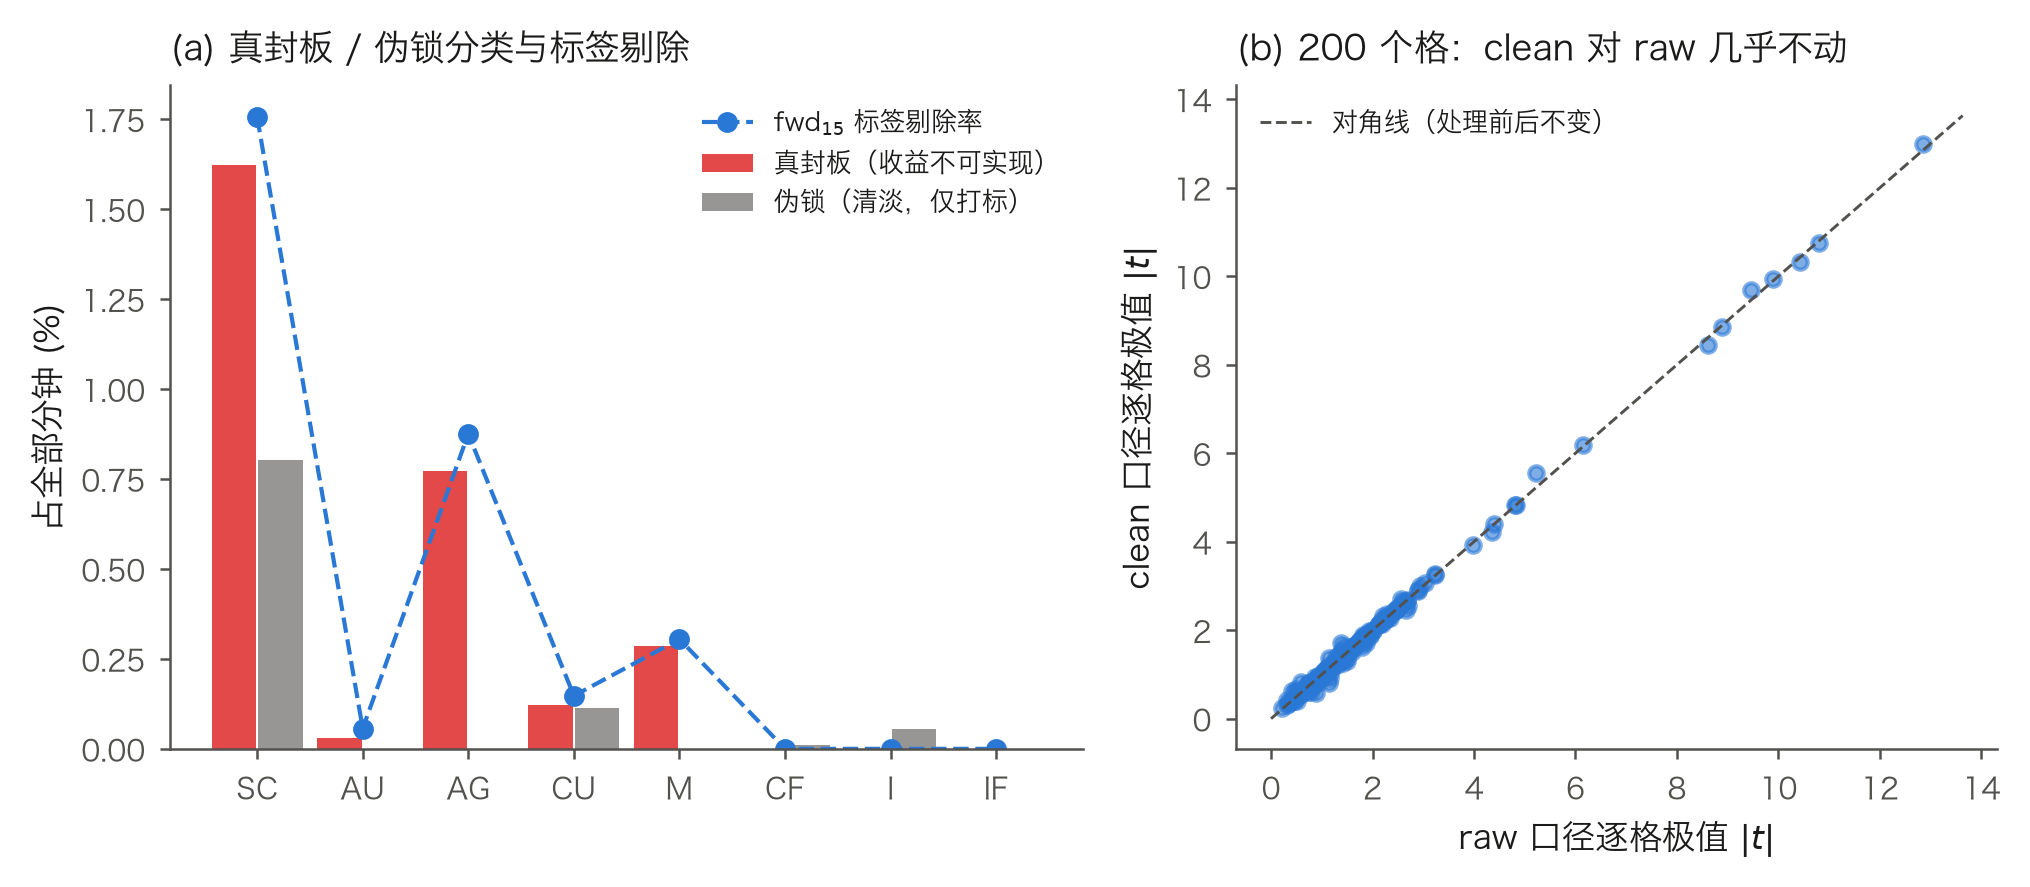
\includegraphics[width=\textwidth]{fig/e1_locked.png}
\caption{涨跌停处理。(a) 分类占比与标签剔除率；(b) 冻结轮 200 个
(信号, 品种) 格的极值 $|t|$：raw 对 clean 几乎全部落在对角线上。
\textbf{纯 Polymarket 极值 $t$ 由 3.240 变为 3.244}：正确的涨跌停处理
不制造任何正结果，只把不可成交的收益从标签中剔掉。}
\label{fig:locked}
\end{figure}

\noindent\textbf{推理：为何剔除不引入选择偏误的方向性担忧。}真封板
剔除的是"标签不可实现"的分钟，同时作用于有利与不利方向（涨停时多头
的浮盈与空头的止损同样无法成交），且剔除决策只依赖价格路径、不依赖
信号取值，故它不会系统性偏向任何信号。图 \ref{fig:locked}(b) 的对角线
散点是这一论断的实证。

%=====================================================================
\section{P5：品种扩展 5 到 8（回应意见 4a）}\label{sec:p5}

CF（棉花）、I（铁矿石）、IF（沪深 300）三品种在 v3 登记表\textbf{早有
事前映射}（分别 13 / 13 / 8 个市场，主题为中美贸易 / 中美贸易 / 台海
风险）、分钟数据已在库，属\textbf{零数据成本、零事后选择}的扩展。

工程纪律：新脚本\textbf{只读 import} 冻结脚本的装配逻辑（分段规则、
z 归一、40 信号定义逐行同源），且先用同一 import 路径重建冻结品种 M
的面板、与存档\textbf{逐值比对}（回归门），通过后才构建新品种。IF 为
纯日盘品种（无夜盘），依赖夜盘的信号（如 X7）退化，评价按实际有限值
计数、\textbf{不虚计分母}。

\begin{table}[h!]\centering\small
\caption{扩展品种的适当口径检验数与极值 $|t|$（clean 标签）。三品种
合计 798 个检验并入扩展主族；纯 PM 侧极值均低于门槛 4.285}
\begin{tabular}{lrrrr}
\toprule
品种 & 检验数 & 极值 $|t|$ & 纯 PM 检验 & 纯 PM 极值 $|t|$ \\
\midrule
CF & 270 & 12.873 & 150 & 2.569 \\
I & 270 & 17.183 & 150 & 2.810 \\
IF & 258 & 9.001 & 138 & 1.966 \\
\bottomrule
\end{tabular}

\end{table}

\noindent\textbf{时间跨度（意见 4c）如实声明}：期货分钟数据止于
2026-07-13，为数据方交付全部，无法延长；由此确认层当前无样本可用，
本轮一切结果为探索层。Polymarket 侧 3 年 8 个月可独立做的检验（概率
校准、外部锚分级）列入第二阶段设计（\code{docs/next\_phase\_design.md}）。

%=====================================================================
\section{P4：分散度矩族——把合并丢掉的信息还原（回应意见 1、2）}\label{sec:p4}

\subsection{诊断}

$N1$ 把 492 个市场压成每分钟 8 个主题数（61:1），且是加权\textbf{均值}
——只保留一阶矩。丢掉的横截面结构包括：市场间\textbf{分歧}（一致小涨与
一个暴涨其余不动，均值可以相同）、\textbf{抵消}（正负创新在求和中
相消）、\textbf{集中度}（信息来自一家独大还是普遍共识）。

\subsection{定义（固定 6 列，维数不随市场数增长）}

设分钟 $t$ 主题内活跃市场集为 $\mathcal{M}_t$（$K_t=|\mathcal{M}_t|$，
$K_t<2$ 时全部置缺失），市场级量取自与冻结面板逐项一致的管道（时点化
准入、结算截断、logit、时点化累计权重）。记定向创新
$x_m=\mathrm{sign}(w_m)\,\Delta\ell_m$、权重绝对值 $a_m=|w_m|$、贡献
$c_m=w_m\Delta\ell_m$、当分钟成交额 $u_m$，则

\begin{align}
\bar x &= \frac{\sum_m a_m x_m}{\sum_m a_m},&
\text{D\_disp} &= \sqrt{\frac{\sum_m a_m (x_m-\bar x)^2}{\sum_m a_m}}
  &&\text{（分歧度）},\\
\text{D\_cancel} &= \frac{|\sum_m c_m|}{\sum_m |c_m|},&
\text{D\_hhi} &= \sum_m \Big(\frac{u_m}{\sum_j u_j}\Big)^2
  &&\text{（抵消存活率、集中度）},\\
\text{D\_sign} &= \frac{\max(K^+,K^-)}{K^++K^-},&
\text{D\_head} &= \frac{\max_m |c_m|}{\sum_m |c_m|}
  &&\text{（符号一致率、头部占比）},
\end{align}
\[
\text{D\_skew} = \frac{\sum_m a_m\big((x_m-\bar x)/s\big)^3}{\sum_m a_m},
\quad s=\text{D\_disp}
\qquad\text{（偏度：极端市场拉动 vs 普遍位移）},
\]
其中 $K^{+}/K^{-}$ 为 $x_m$ 取正 / 负的市场数。

\textbf{算例（读 D\_cancel）}：两市场贡献 $c_1=+0.4$、$c_2=-0.3$，则
D\_cancel $=|0.1|/0.7\approx0.14$——毛信念变动的 86\% 在合并中被抵消，
这正是意见 1 所指"合并丢信息"的量化形态；D\_cancel 把它变成了可检验
的列。

\subsection{纪律与结果}

方向先验\textbf{事前注册为 0}（六列均无"该正该负"的经济先验，如实登记、
只做双侧检验；仅 D\_disp 的波动通道注册为正）。固定维数使检验数受控：
78 个格、354 个适当检验，如实并入扩展主族。

\begin{table}[h!]\centering\small
\caption{分散度矩族 $|t|$ 前 8 格。\textbf{两个一致率口径勿混}：表内
列为\emph{该格六视界内}的符号一致率；正文引用的 58\% 则是
D\_hhi\_metal\_price \emph{信号跨品种}（AU/AG）$\times$6 视界共 12 个
IC 的一致率（纯噪声期望约 57\%）。极值格 $|t|=3.994<4.285$：幅度不足，
且信号层面方向不连贯}
\begin{tabular}{lrrr}
\toprule
信号$\cdot$品种 & 非零占比 & 极值 $t$（带符号） & 六视界内一致率 \\
\midrule
D\_hhi\_metal\_price$\cdot$AG & 100.0\% & -3.994 & 83\% \\
D\_head\_share\_taiwan\_risk$\cdot$IF & 100.0\% & -3.853 & 100\% \\
D\_disp\_metal\_price$\cdot$AU & 43.1\% & -3.078 & 50\% \\
D\_hhi\_us\_china\_trade$\cdot$CF & 100.0\% & -2.605 & 100\% \\
D\_sign\_ratio\_us\_china\_trade$\cdot$I & 100.0\% & +2.420 & 100\% \\
D\_cancel\_us\_china\_trade$\cdot$I & 100.0\% & +2.259 & 100\% \\
D\_hhi\_us\_china\_trade$\cdot$I & 100.0\% & -2.182 & 100\% \\
D\_skew\_metal\_price$\cdot$AU & 43.1\% & -2.158 & 100\% \\
\bottomrule
\end{tabular}

\end{table}

\noindent\textbf{推理}：若"合并丢掉的信息"里藏有可交易信号，这 6 列
应当至少有一列跨过门槛且方向连贯。实测最强格幅度不足、符号一致率与
纯噪声无异，故\textbf{意见 1/2 所指的信息损失确实存在（构造上可量化），
但还原之后仍不构成分钟级 alpha}——这本身就是对意见 1/2 的完整回答。
第二阶段将做更深的去聚合（头 / 尾分层、旗舰市场、按 as-of
\code{close\_at} 的生命周期分层）。

%=====================================================================
\section{P3：top-bottom 分位与成本净边界（回应意见 5、6）}\label{sec:p3}

\subsection{分档（严格历史断点，防前视）}

对信号 $s$、交易日 $d$：断点取此前 20 个交易日\textbf{非零}取值的
十分位
\[
Q^{(d)}_{j} = \mathrm{quantile}_{j/10}
\big(\{s_u \ne 0:\ u\in \text{日 } d{-}20..d{-}1\}\big),
\quad j=1..9,
\]
当日各 bar 按 $Q^{(d)}$ 归档得 $q_t\in\{1..10\}$；零值与真封板分钟不
参与。断点只用 $d$ 之前的数据，当日任何信息不进入当日分档。

\subsection{三套判据}

\textbf{(i) 多空价差}：$\mathrm{LS}_k(d)=$ 档 10 当日均值 $-$ 档 1
当日均值（$\mathrm{fwd}^{\mathrm{clean}}_k$），对日序列做 HAC(5) $t$：
\[
t = \frac{\overline{\mathrm{LS}}}{\sqrt{\hat\Omega/n}},\qquad
\hat\Omega = \hat\gamma_0 + 2\sum_{l=1}^{5}
\Big(1-\frac{l}{6}\Big)\hat\gamma_l,
\]
$\hat\gamma_l$ 为日序列去均值后的 $l$ 阶自协方差（Newey--West，
Bartlett 权）。

\textbf{(ii) 单调性}：pooled 档均值对档序的 Spearman $\rho$，与逐日
"档序回归斜率"的日间 $t$；两者同号且斜率 $|t|\ge2$ 记单调。单调性
回答 IC 回答不了的问题：IC 大但档间不单调，说明关联由少数极端点承载、
不可作分档组合交易。

\textbf{(iii) 成本净边界}（1 分钟再平衡的真实策略，无重叠）：状态
$s^{*}_t=+1$（档 10）、$-1$（档 1）、$0$（其余），
\[
\text{日毛利} = \sum_{t\in d} s^{*}_t\,\mathrm{fwd}_{1,t},\qquad
\text{日成本} = \frac{c}{2}\sum_{t\in d} |s^{*}_t - s^{*}_{t-1}|,\qquad
c = 16\ \text{bp（冻结的完整换手成本）},
\]
仓位变动一个单位记半次完整换手。盈亏平衡倍数 $=$ 日成本 $/$ $|$日毛利$|$。

\subsection{结果}

215 个 (信号, 品种) 对中 114 个过覆盖门（两端极端档非空的交易日
$\ge60\%$）：

\begin{itemize}
\item 注册终点 $k{=}15$：114 个检验，$\max|t|=3.039$，无一过门槛
  （纯 PM 子集 $\max|t|=1.877$）；
\item 单调：仅 5/114；
\item \textbf{成本后净收益为正：0/114}；盈亏平衡倍数中位
  \textbf{47.5}。
\end{itemize}

\begin{table}[h!]\centering\small
\caption{分位检验 $|$LS $t|$ 前 10 对。即便统计上最强的格，日成本也
数十倍于日毛利}
\setlength{\tabcolsep}{4pt}
\begin{tabular}{lrrrrrr}
\toprule
信号$\cdot$品种 & LS$_{15}$(bp) & $t$ & 单调 & 日毛利(bp) & 日成本(bp) & 日净(bp) \\
\midrule
C4$\cdot$AG & -12.52 & -3.04 & 否 & +1.0 & 155.4 & -154.4 \\
C6$\cdot$IF & -4.70 & -2.29 & 否 & -2.2 & 155.9 & -158.1 \\
C5$\cdot$AG & -16.37 & -2.24 & 否 & -7.0 & 168.4 & -175.4 \\
C4$\cdot$IF & -3.61 & -2.18 & 否 & +0.6 & 142.0 & -141.4 \\
C6$\cdot$I & +4.55 & +2.12 & 否 & +4.5 & 202.7 & -198.2 \\
C9$\cdot$SC & -8.19 & -2.07 & 否 & -12.2 & 236.5 & -248.7 \\
C1$\cdot$AG & -5.50 & -2.05 & 否 & -33.8 & 313.3 & -347.1 \\
C8$\cdot$SC & +9.33 & +1.97 & 是 & +17.2 & 184.7 & -167.5 \\
C9$\cdot$AG & -10.12 & -1.97 & 否 & -4.6 & 117.4 & -122.0 \\
N1$\cdot$CU & -2.56 & -1.88 & 否 & -0.3 & 73.2 & -73.5 \\
\bottomrule
\end{tabular}

\end{table}

\begin{figure}[h!]\centering
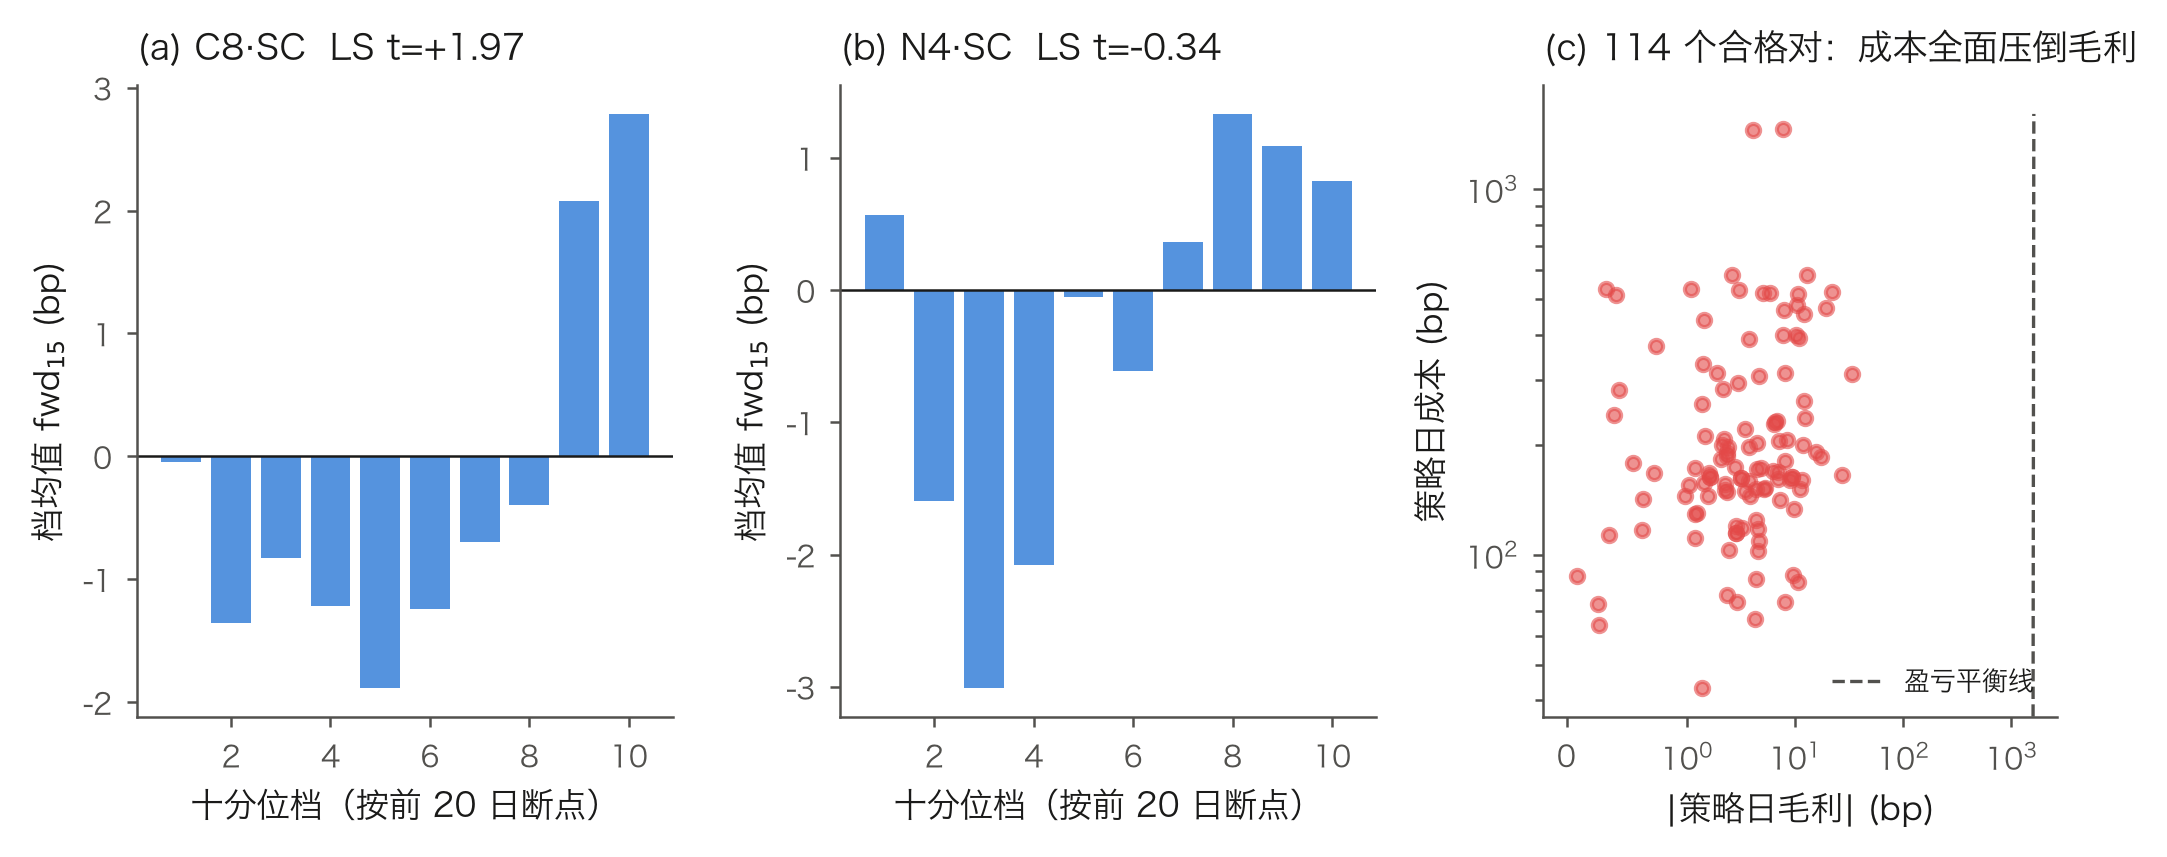
\includegraphics[width=\textwidth]{fig/e2_quantile.png}
\caption{分位与成本。(a)(b) 两个代表格的十分位收益剖面（C8$\cdot$SC
虽两端抬升但 LS $t$ 仅 $+1.97$；N4$\cdot$SC 无单调结构）；(c) 114 个
合格对的策略日毛利对日成本：全部远在盈亏平衡线（虚线）之外——毛利
1--30 bp 量级，成本 100--1000 bp 量级。}
\label{fig:quantile}
\end{figure}

\noindent\textbf{推理：分位透镜为何是对 IC 透镜的实质补充。}IC 只度量
排序相关，不度量可交易性；分位组合把信号变成真实持仓，于是换手与成本
自动进入。本轮的答案是两层的：统计层面 $\max|t|=3.04$ 不过门槛（与 IC
结论一致）；经济层面即便统计过了，1 分钟频率的换手使成本吞掉毛利的
数十倍——\textbf{分钟级不可交易不是"差一点"，是差一个数量级以上}。

%=====================================================================
\section{P6：因子质量七关门控（回应意见 6）}\label{sec:p6}

"现有 40 个因子对质量没有要求"如实承认。下一阶段准入制度化为七关，
全部机械可查、任一不过即留探索层：

\begin{enumerate}
\item \textbf{预注册}：经济假说与预期符号已在计算前登记；
\item \textbf{覆盖}：非零分钟占比 $\ge1\%$ 且日均有效观测 $\ge30$；
\item \textbf{正交增量}：对期货量价四因子（mom / rv / volu / amt 的
  $z$ 分数）\textbf{逐日日内}残差化后，残差 RankIC 的日间 $|t|\ge2$；
\item \textbf{单调}：P3 分位单调判据（$k{=}15$）；
\item \textbf{稳定}：跨品种 IC 符号一致率 $\ge60\%$；
\item \textbf{成本}：P3 策略净收益在至少一个品种为正；
\item \textbf{无前视}：截去尾部交易日重算，公共区间取值逐值不变
  （构造只依赖 $\le t$ 的信息的机械证明）。
\end{enumerate}

\begin{table}[h!]\centering\small
\caption{首批候选（6 个分散度因子）的七关矩阵：无一全过（各过
3--4 关），全部留探索层。门控真实生效，不是摆设}
\setlength{\tabcolsep}{4pt}
\begin{tabular}{lcccccccr}
\toprule
因子 & 1 预注册 & 2 覆盖 & 3 正交增量 & 4 单调 & 5 稳定 & 6 成本 & 7 无前视 & 通过 \\
\midrule
D\_disp & \ding{51} & \ding{51} & $\times$ & $\times$ & \ding{51} & $\times$ & \ding{51} & 4/7 \\
D\_cancel & \ding{51} & \ding{51} & $\times$ & $\times$ & \ding{51} & $\times$ & \ding{51} & 4/7 \\
D\_hhi & \ding{51} & \ding{51} & $\times$ & $\times$ & $\times$ & $\times$ & \ding{51} & 3/7 \\
D\_sign\_ratio & \ding{51} & \ding{51} & $\times$ & $\times$ & \ding{51} & $\times$ & \ding{51} & 4/7 \\
D\_head\_share & \ding{51} & \ding{51} & $\times$ & $\times$ & $\times$ & $\times$ & \ding{51} & 3/7 \\
D\_skew & \ding{51} & \ding{51} & \ding{51} & $\times$ & $\times$ & $\times$ & \ding{51} & 4/7 \\
\bottomrule
\end{tabular}

\end{table}

\noindent\textbf{推理：门控与检验族的关系。}门控不产生对外检验、不进
任何族；它的作用是把进入确认层的假设数从"任意多"压到"极少数且各有
事前符号"，从而使确认层（未触碰样本上一因子一预约）的多重检验负担
合法地小。反过来说：\textbf{绝不在同一 125 天样本上先用门控筛选、再用
更松门槛判定}——那是把筛选信息用了两次。

%=====================================================================
\section{扩展主族总账与结论}\label{sec:ledger}

\subsection{总账}

扩展主族 $=$ v3 冻结轮全部检验 $+$ 三个新块，门槛按
$\Phi^{-1}(1-\alpha/2m)$ 随总数 $m$ 上升：

\begin{table}[h!]\centering\small
\caption{扩展主族总账。门槛从 4.146 升至 \textbf{4.285}：扩展使判定更
严而非更松，这本身就是反操纵证明}
\begin{tabular}{lrr}
\toprule
构成 & 检验数 & Bonferroni 门槛 \\
\midrule
v3 冻结轮（原样保留） & 1,476 & 4.146 \\
$+$ 扩展品种 CF/I/IF（P5） & 798 & \\
$+$ 分散度矩族（P4） & 354 & \\
$+$ 分位注册终点 $k{=}15$（P3） & 114 & \\
\midrule
\textbf{扩展主族合计} & \textbf{2,742} & \textbf{4.285} \\
\bottomrule
\end{tabular}

\end{table}

\begin{figure}[h!]\centering
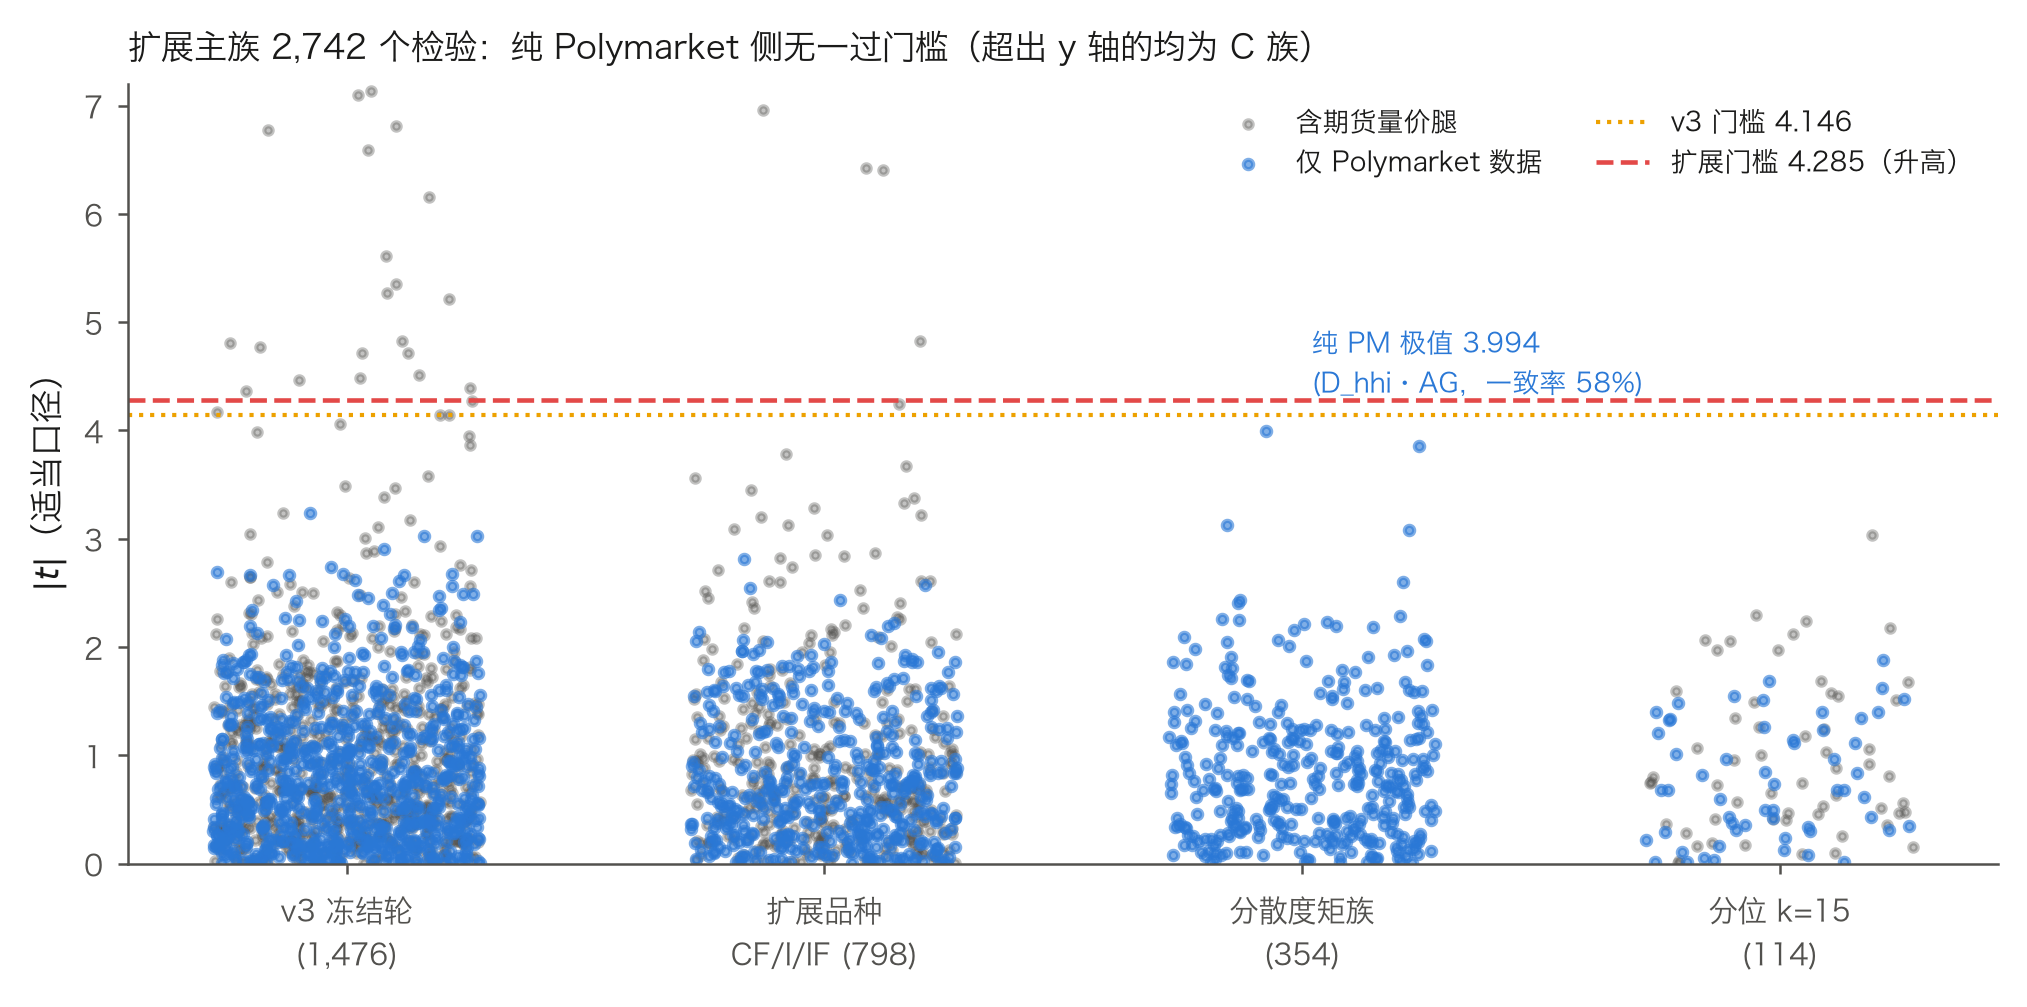
\includegraphics[width=\textwidth]{fig/e3_ledger.png}
\caption{扩展主族 2{,}742 个检验的全景。蓝点 $=$ 仅用 Polymarket 数据
（含分散度矩族），灰点 $=$ 含期货量价腿；红虚线为扩展门槛 4.285。
纯 Polymarket 侧 1{,}646 个检验极值 3.994、无一过线；超出门槛的全部为
C 族（期货腿）。}
\label{fig:ledger}
\end{figure}

\subsection{结论}

\begin{enumerate}
\item 通过门槛的 73 个检验\textbf{全部来自 C 族}（含期货量价腿），
  归因结构与冻结轮完全一致：显著性来自期货自身的短期反转，不来自
  Polymarket；
\item \textbf{纯 Polymarket 侧 1{,}646 个检验，$\max|t|=3.994$
  （D\_hhi$\cdot$AG；该信号跨品种$\times$视界的符号一致率仅 58\%），
  通过 0 个}；
\item 分位透镜给出更彻底的经济否定：净收益为正 0/114，盈亏平衡倍数
  中位 47.5；
\item 涨跌停正确处理后核心数字不动（3.240 $\to$ 3.244），证明结论
  不依赖标签口径的选择。
\end{enumerate}

\paragraph{诚实声明。}本轮全部结果计算于同一段 125 天样本，属
\textbf{探索层}；确认必须等未触碰样本（期货分钟库止于 2026-07-13，
新样本尚不存在、可能不再交付）。本研究的对外结论保持为冻结轮的诚实
否定。六个分散度因子未通过质量门控，同样如实报告——\textbf{门槛与
门控对自己的新构造同样无情，正是这套纪律可信的原因}。

%=====================================================================
\section{复现}

\begin{table}[h!]\centering\small
\caption{扩展轮复现命令链（顺序即依赖）}
\begin{tabular}{p{5.6cm}p{7.8cm}}
\toprule
步骤 & 命令 / 产物 \\
\midrule
P1 映射与预注册 & \code{v4\_mapping\_strength.py $\to$
  taxonomy / tier\_registry / prereg\_signs} \\
P1 冻结账本 & \code{v4\_freeze\_mapping.py $\to$
  freeze/manifest\_v2.json} \\
P2 评价引擎（含回归门） & \code{v4\_signal\_grid.py $\to$
  signal\_grid\_clean / locked\_impact} \\
P5 面板扩展（含回归门） & \code{v4\_panel\_build.py $\to$
  panel\_\{CF,I,IF\}} \\
P4 分散度构建与评价 & \code{v4\_market\_dispersion.py $\to$
  v4\_dispersion\_eval.py} \\
P3 分位检验 & \code{v3\_quantile.py $\to$ quantile\_grid} \\
P6 质量门控 & \code{next\_factor\_gate.py $\to$ quality\_scorecard} \\
关键数字 & \code{v4\_key\_numbers.py $\to$
  docs/concise/key\_numbers\_v2.json} \\
本文图表 & \code{v4\_ext\_figures.py / make\_ext\_report.py} \\
本文编译 & \code{xelatex main.tex}（两遍） \\
\bottomrule
\end{tabular}
\end{table}

\vspace{1em}
\noindent\rule{\textwidth}{0.4pt}\\
\small 设计文档：\code{docs/next\_phase\_design.md}（含第二阶段五项
与否决清单）。\\
主报告：\code{docs/cn\_futures\_polymarket\_concise.pdf}（37 页，其
§扩展轮为本文的摘要版）。\\
分支 \code{feat/cn-futures-polymarket}。

\end{document}
